\chapter{Metodologia} \label{cap:metodologia}


\section{Análise de Contexto}

\subsection{Definições do Sistema}

\subsubsection{Visão Geral da Arquitetura}



O sistema será composto por quatro partes.

\begin{enumerate}
	\item Aplicativo Android que será utilizado como a interface homem máquina, além de contribuir com o monitoramento dos sensores e ser responsável por disparar requisições de avisos para o servidor em nuvem.
	\item Hardware responsável por monitorar as forças do veículo e auxiliar na detecção dos eventos de interesse.
	\item Servidor em nuvem responsável por receber os dados, armazena-los e disponibilizar o acesso das informações adquiridas através de uma interface web.
	\item Interface Web será responsável por mostrar de forma intuitiva os dados coletados pelo sistema.
\end{enumerate}


\subsubsection{Funcionamento}

O sistema contará com um aplicativo Android capaz de realizar cadastro de informações sobre o usuário para identificação e rastreio, juntamente será utilizado os sensores disponíveis no celular para o monitoramento, qualquer variação muito elevada será disparada uma requisição HTTP para o servidor. Os demais aplicativos da proximidade serão alertados do incidente com isto poderão visualizar informações essências sobre o usuário acidentado podendo se deslocar até o local e efetuar chamadas.

No veiculo será acoplado um sistema embarcado para auxiliar nas medições dos sensores porem utilizando os próprios sensores do embarcado, quando houver alguma variação brusca o embarcado emitira um sinal via Bluetooth para o aplicativo onde será disparando uma requisição HTTP para o servidor.

O servidor será responsável pela persistência dos dados recebidos dos aplicativos, e gerenciamento dos alertas para os dispositivos próximos , além de disponibilizar informações através de requisições HTTP.

\subsubsection{Atores}

Os sistemas como um todo terá os 2 atores humano e sistêmicos.
O Ator humano é responsável, pela interação dentro do aplicativo e navegação dentro da interface web.

Já o Ator sistêmico será  todas as mensurações dos sensores além de todas as requisições feitas entre as  4 interfaces já citadas.



\clearpage
\subsubsection{Interfaceamento entre as partes}

O sistema terá como interfaceamento entre as partes  protocolos de comunicação HTTP e bluetooth , o diagrama abaixo demonstra a interface geral do sistema



\begin{figure}[H]

 \caption{Interface do sistema}
 \centering
  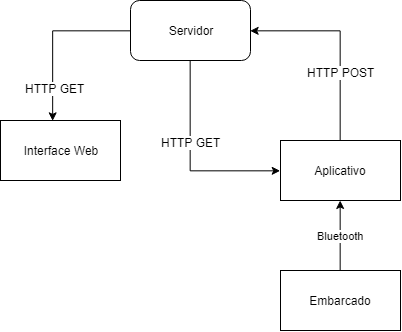
\includegraphics[width=100mm]{images/Cap3/diagrama_funcionamento.png}
  
    
\end{figure}




\subsection{Condições Restritivas}
\subsubsection{Custos}

\begin{table}[h!]
  \begin{center}
    \caption{Tabela contendo o custo do projeto }
    \label{tab:table1}
    \begin{tabular}{l|S|r}
      \textbf{Equipamento} & \textbf{Custo} \\
    
      \hline
      Celular & R\$ 200  \\
      ESP32 & R\$ 40 \\
      MPU6050 & R\$15 \\
      Servidor & R\$ 35 \\
      
    \end{tabular}
  \end{center}
\end{table}

\clearpage
\subsubsection{Recursos}

\begin{enumerate}
    \item Celular Android 5.0 ou superior
    \item Placa embarcada ESP 32
    \item Modulo Acelerometro MPU6065
    \item Servidor em nuvem
\end{enumerate}


\subsubsection{Ambientais}
Não se aplica
\subsubsection{Físicas e tecnológicas}
O sistema é restritivo aos seguintes itens:
\begin{enumerate}
    \item Modelo do smartphone utilizado;
    \item Duração da bateria do smartphone;
    \item Dependência de rede móvel;
\end{enumerate}

\subsubsection{Energização}

\subsubsection{Interferências devido ao meio}
A aquisição de dados não deverá sofrer grandes interferências, entretanto as comunicações podem ser comprometidas. A grande presença de ruído eletromagnético, bem como a presença de diversas redes wireless no meio podem atrapalhar ou mesmo anular a comunicação entre os dispositivos .

\subsection{Benefícios e Impactos}
\subsubsection{Econômicos}
Não se aplica
\subsubsection{Operacionais}
\subsubsection{Estratégicos}
\subsubsection{Políticos}
Não se aplica
\subsubsection{Sociais}


\section{Análise Funcional e de Requisitos}
\subsection{Lista de funcionalidades}
\subsection{Comunicação}
\subsection{Processamento}
\subsection{Interface Homem-Máquina}
\subsection{Sistemas Controlados Automaticamente}
teste
\subsection{Aquisição de dados}
\subsection{Atuação}


\section{Análise da Arquitetura do Sistema}
\subsection{Hardware}
\subsubsection{Diagrama de Blocos}
\subsubsection{Diagrama de Fluxo para Firmware}

\subsection{Software}
\subsubsection{DER/MER}


\begin{figure}[H]

 \caption{Diagrama de entidade e relacionamento}
 \centering
  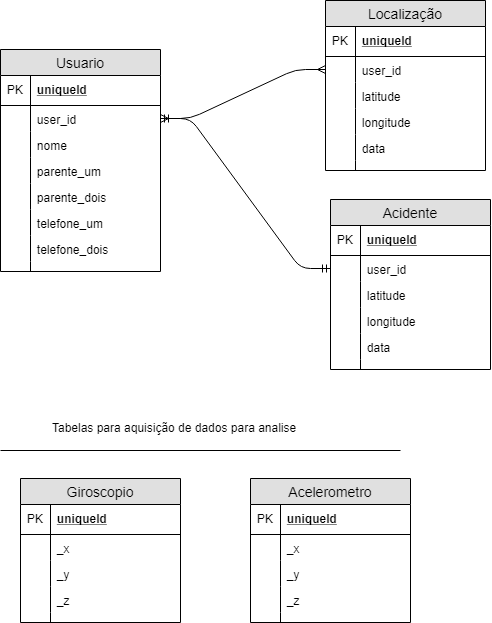
\includegraphics[width=100mm]{images/Cap3/Diagrama_ER_f.png}
  
    
\end{figure}




\subsubsection{Use Case}
\subsubsection{Diagramas de Sequência}
\subsubsection{Diagramas de Classe}

